% Migrated from studies/bin_packing/project2-writeup/p2_writeup.tex
\section{Bin Packing}
\noindent This report analyzes the waste generated by five bin packing
	algorithms: \emph{Next Fit, First Fit, Best Fit, First Fit Decreasing}
	and \emph{Best Fit Decreasing}.


\subsection{Introduction}
The \emph{Bin Packing} problem is an optimization problem wherein items of
different sizes must be \emph{packed} into a finite number of \emph{bins} with
a certain capacity. Formally, take $I = \left\{i_1, \dots i_n \right\}$ to be
a set of $n$ items, where for each $i_k \in I$, a function $s$
\begin{align*}
	s \colon  I & \to (0, 1]     \\
	i_k         & \mapsto s(i_k)
\end{align*}
denotes the size of the item. We want to know, for a set of bins
$B = \left\{ b_1, \dots, b_m \right\}$ with initial capacities $c(b_i) = 1$ for
all $i \in \{1, \dots, m\}$, the miniumum number of bins required to pack all
$|I|$ items.

Despite its simple nature, the problem is computationally
\textbf{NP-Hard}, meaning that its incredibly unlikely a polynomial time
algorithm exists to \emph{optimally} solve it. There are, however, many
approximation algorithms we can use to \emph{approximate} bin packing, of which
five will be discussed in later sections.

\subsubsection{Waste}
The goal of each of the experiments is to provide empirical evidence for
estimating the \emph{Waste} of a bin-packing algorithm. Let $\bbI$ denote the
set of all sequences of valid items and $\bbA$ the set of all algorithms.
\begin{equation*}
	W \colon (\bbA, \bbI) \to \bbR^+ \cup \left\{ 0 \right\}
\end{equation*}
be the waste of an algorithm, $A$,  where for a set of items $I$:
\begin{equation*}
	W(A, I) = |\text{Bins Used by }A| - \sum_{i \in I} s(i)
\end{equation*}
We define waste as to compare approximation algorithms, instead of those that
find the optimal solution. This is more valuable to reasoning which of the
superceding algorithms is best, since computing an approximation ratio
of an algorithm
\begin{equation*}
	\frac{ALG(I)}{OPT(I)}
\end{equation*}
is contingent on knowing the optimal solution, which takes exponential time
to compute.

\subsubsection{Data Structures}
Traditional \emph{Best Fit} and {Next Fit} variations run in
$\mcO(n^2)$ time. We utilize a \emph{Zip Zip Tree} to optimize both algorithms.
Formally, a \emph{Zip Zip Tree} is a binary search tree where every node has a
numeric \emph{rank}, and the tree is max-heap ordered with respect to \emph{rank}.

\emph{Zip Trees}, in their very nature, are constructed in such a way as to
emulate a perfect binary tree. Theory tells us that perfect binary tree's have
height $h = \log_2 (n)$, for $n$ vertices. \emph{Zip Trees} invert this fact, and
let \emph{rank} be a geometric random variable with success probability
$p = \frac{1}{2}$. To break collisions, we let \emph{rank} be a tuple $(r_1, r_2)$
where

\begin{align*}
	r_1 & \sim Geom(\frac{1}{2}), & \mcO(\log \log n)   \\
	r_2 & \sim Unif[0, \log^c n], & \mcO(c \log \log n)
\end{align*}
and compare nodes lexigraphically.
\emph{Zip Trees} support \texttt{insert}, \texttt{find}, and \texttt{delete}
with help from the \texttt{zip} operation. \emph{Zipping} and \emph{Unzipping}
preserve the order and max-heap properties. \emph{Zip Trees} are very efficient andeasyto implement, and, arguably more importantly, are isomorphic to skip-lists of
which were implemented in \emph{Project 1: Sorting}.

\subsection{Next Fit}

\emph{Next Fit} is the most original hueristic aprroximation algorithm.
It is simply:
\begin{itemize}
	\item Try to place item $i$ into bin $b$
	\item If it fits, put it there.
	\item If not, start a new bin.
\end{itemize}
The approximation ratio for Next Fit is $SOL = k < 2M$, where $M$ is the optimal number of bins. The \emph{Waste} grows linearly
\begin{figure}[H]
	\centering
	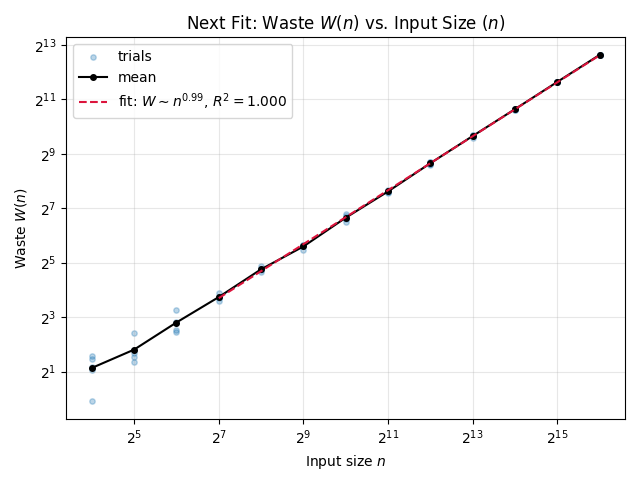
\includegraphics[width=0.7\textwidth]{photos/nf.png}
	\caption{Next Fit Waste}
	\label{fig:nf}
\end{figure}
as noted by the figure above. This is in direct agreement with the
approximation ratio since there is $N$ waste for an input size of $N$,
meaning we are bounded by $N$ extra buckets in the worst case (all waste
requires a new bucket). This is exactly the bound above,
\begin{equation*}
	W(NF, A) \propto N, \qquad SOL = k < 2N
\end{equation*}

\subsection{First Fit} \label{sec:ff}
The \emph{First Fit} algorithm is as follows
\begin{itemize}
	\item Scan throuh bins $b_1, b_2, \dots b_i$
	\item Place item $i$ in the first bin that is large enought to hold it,
	      $c(b_i) \geq s(i)$
	\item Create a new bin $b_{i + 1}$ if there are \emph{no} bins
	      that are large enough
\end{itemize}
From the lecture slides, we know that for $M$ the number of bins to optimally
pack $I$ items, the approximation ratio of First Fit, $FF$, is
\begin{equation*}
	SOL_{FF} = \lceil 1.7M \rceil.
\end{equation*}
\begin{figure}[ht]
	\centering
	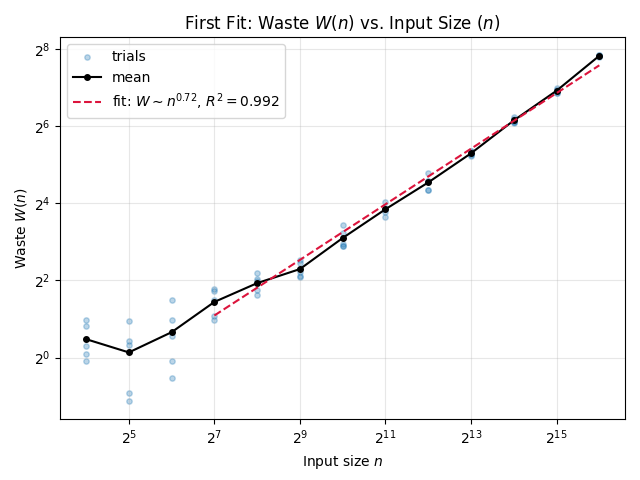
\includegraphics[width=0.7\textwidth]{photos/ff.png}
	\caption{First Fit Waste}
	\label{fig:ff}
\end{figure}

We start the best fit line at $2^7$ samples to eliminate the noise from smaller
inputs. We see that the Waste is of order $\mcO(n^{0.72})$, which is reflective
of it's theoretical result. For a large $N$, In the worst case, we let
each bit of waste require a new bucket, and as such we would be bounded by
$N_{OPT} + 0.72N_{FF} = 1.72N$, supporting the theoretical result.

\newpage
\subsection{Best Fit} \label{sec:bf}
\emph{Best Fit} works as follows:
\begin{itemize}
	\item For item $i$, find the bin $b^*$ with the least remaining capacity that still fits:
	      \begin{equation*}
		      b^* = \argmin_{b} \left\{ c(b) - s(i) \;\middle|\; c(b) \geq s(i) \right\}
	      \end{equation*}
	      where $c(b)$ is the remaining capacity of bin $b$ and $s(i)$ is the size of item $i$.
	\item If no such bin exists, open a new one.
\end{itemize}
The theoretical approximation ratio for \emph{Best Fit}, $BF$, as suggested
by Dosa and Sgall (2014), is
\begin{equation*}
	SOL_{BF} = k \leq \lfloor 1.70M \rfloor
\end{equation*}
\begin{figure}[H]
	\centering
	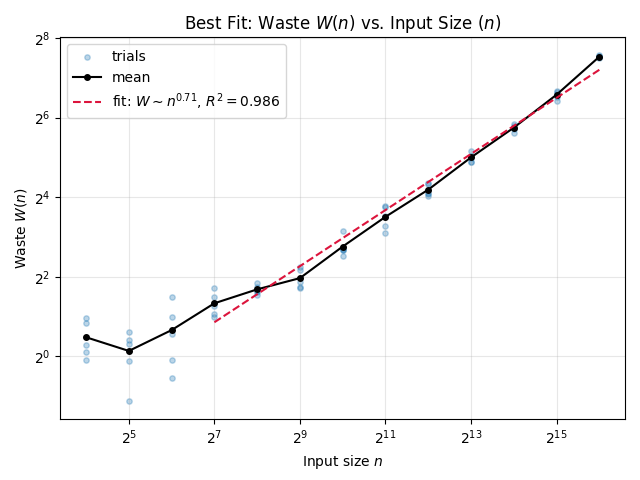
\includegraphics[width=0.7\textwidth]{photos/bf.png}
	\caption{Best Fit Waste}
	\label{fig:bf}
\end{figure}
We once again begin fitting the data at $2^7$ samples to reduce noise. Notice that
there is less variance amoung the trials (less spread out) than in First Fit,
but our $R^2$ value is lower. This suggests that Best Fit may be a more
consistent option than first fit. We see that the empirical waste follows
$\mcO (n^{0.71})$, and by the same reasoning as \emph{Next Fit} and
\emph{First Fit}, for a large $N$ support
\begin{equation*}
	1 N_{OPT} + 0.71N_{BF} = 1.71N
\end{equation*}
which is a bit above the suggested lower bound, but close enough to call for
statistical variance.


\subsection{First Fit Decreasing}
The \emph{First Fit Decreasing} algorithm is
\begin{itemize}
	\item Sort the items $I$ in descending order
	\item Run the \emph{First Fit} algorithm [\ref{sec:ff}] on $I$
\end{itemize}

Compared to all previous algorithms (\emph{Next Fit}, \emph{First Fit} and
\emph{Best Fit}), \emph{First Fit Decreasing} has a wildly different
waste-complexity.

\begin{figure}[H]
	\centering
	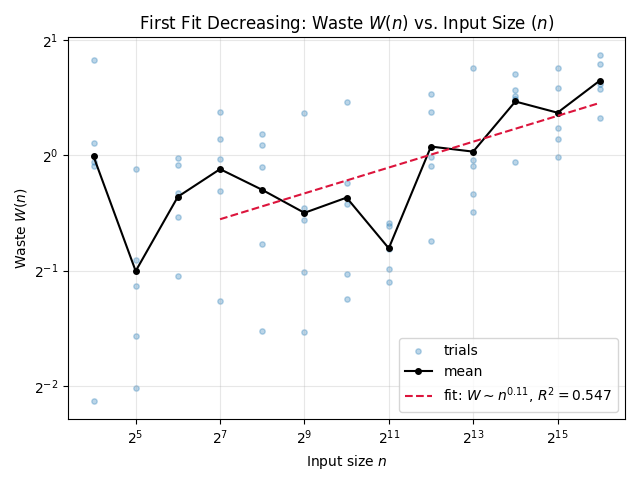
\includegraphics[width=0.8\textwidth]{photos/ffd.png}
	\caption{First Fit Decreasing Waste}
	\label{fig:ffd}
\end{figure}

Note that the scaling of the axis: the trials would appear much closer together
if the scaling was the same as the first three algorithms. The empirical waste
complexity is $\mcO(n^{0.11})$, which is much must better than any previous
algorithm. Sorting the list in decreasing order lets us more tightly pack (
put more items in)  the first bins, which has a profound impact on the waste.
We should note, however, that \emph{FFD} required us to \textbf{sort} the
input, which is at best $\mcO (n \log n)$ using Tim-Sort. While the waste was
significantly lower, the runtime might not be.

\subsection{Best Fit Decreasing}\label{sec:bfd}

The \emph{Best Fit Decreasing} algorithm is
\begin{itemize}
	\item Sort the items $I$ in descending order
	\item Run the \emph{Best Fit} algorithm [\ref{sec:bf}] on $I$
\end{itemize}

In excactly the same way as \emph{First Fit Decreasing}
\emph{Best Fit Decreasing} has a very very low waste-complexity.

\begin{figure}[H]
	\centering
	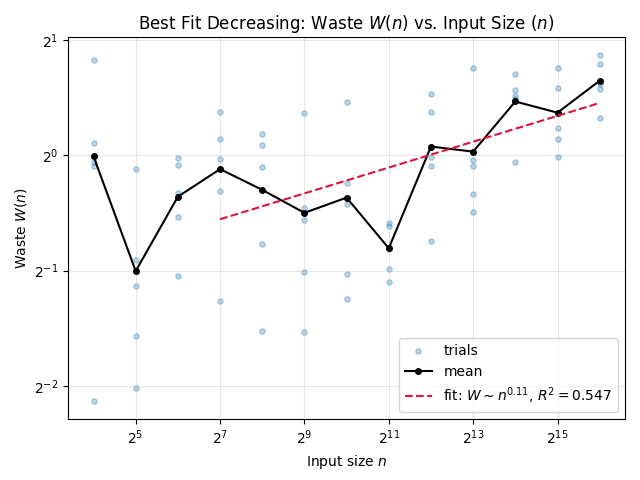
\includegraphics[width=0.8\textwidth]{photos/bfd.png}
	\caption{Best Fit Decreasing Waste}
	\label{fig:bfd}
\end{figure}

Where the empirical waste is order $\mcO(n^{0.11})$, the same as in \emph{FFD}.
Interestly enough, the plots are \emph{exactly} the same. Even considering the
individual trials, both graphs are identical. I conjecture that this is no
coincidence. That, in fact, each bin may not be filled the exact same way, but the number
of bins is always the same, given the input distribution. (expanded
upon in [\ref{sec:conc}]).

\subsection{Conclusion}\label{sec:conc}

There are two factors to consider when determining the \emph{best} bin-packing
algorithm: \emph{run time} and \emph{waste}.

Let's first rule out \emph{Next Fit} since it's empirical waste complexity
was $\mcO(n^{0.99})$, satisfying its theoretical approximation ratio of $2M$ for
$M$ optimal bins. It's simply not a good enough approximation, even though the
run-time of the algorithm is the fastest at $\mcO(n)$.

\emph{First fit} and \emph{Best fit} perform quite well, with \emph{best fit}
slightly edging out the \emph{first fit} with waste complexity
$\mcO_{FF}(n^{0.72}) \; vs. \; \mcO_{BF}(n^{0.71})$. This makes sense since
\emph{best fit} should, in theory, have tighter packings.

The real decision is between \emph{First fit decreasing} and
\emph{best fit decreasing}. Both of the graphs (figures \ref{fig:ffd},
\ref{fig:bfd}) are nearly identical, with empirical waste complexity
$\mcO(n^{0.11})$ in both cases. As conjectured in section [\ref{sec:bfd}],
this is likely not a coincidence: once the input is sorted in decreasing
order, the largest items dominate the packing structure.
Since both algorithms have the same waste complexity, we have to pivot to
runtime analysis. \emph{Both} algorithms incur a $\mcO(n \log n)$ sort cost
using \texttt{Tim Sort} to sort the items in decreasing order. \emph{BFD} and
\emph{FFD} both use a \texttt{Zip Zip Tree}, but the augments are different.
Asymptotically, the two are equivalent, but \emph{FFD} may have a smaller constant
factor since it accepts the \emph{first} feasible bin, rather than the tightest fit one.
As such \textbf{First Fit Decreasing} is the best bin-packing algorithm.





